\subsection{联合分布与边缘分布}\label{sec:4.1}
前几章研究的模型只涉及一个随机变量，称为单变量模型（univariate model）. 本章讨论包含多个随机变量的模型，称为多变量模型（multivariate model）.

在实验中，我们很少只观测一个值. 例如，研究某个总体的健康状况时，如果只测量一个人的体重，这个实验的规模实在很小. 若测量若干人的体重，就有若干个随机变量，每个人对应一个. 或者，也可以为每个人测量若干特征，例如体重、体温、身高和血压；每个特征都对应一个随机变量. 因此，需要能够处理多个随机变量的模型. 本章前几节主要讨论两个随机变量的模型，即二元模型（bivariate model）.

回顾\autoref{def:1.4.1}，随机变量是从样本空间 $S$ 到实数集的函数. 由若干随机变量组成的向量也可以类似地定义.
\begin{definition}\label{def:4.1.1}\index{SI0871@随机向量}
一个 $n$ 维随机向量（random vector）是从样本空间 $S$ 到 $\mathbb R^n$（$n$ 维欧几里得空间）的函数.
\end{definition}
例如，若为样本空间的每个点指定平面 $\mathbb R^2$ 中的一个有序对 $(x,y)$，就定义了二维（或二元）随机向量 $(X,Y)$. 下例说明这一过程.
\begin{example}[骰子的样本空间]\label{ex:4.1.2}
掷两颗公平骰子的样本空间包含 36 个等可能的点，已在\autoref{ex:1.3.10} 中介绍. 点 $(3,3)$ 表示两颗骰子均出现 3；点 $(4,1)$ 表示第一颗出现 4，第二颗出现 1，等等. 现在为每个样本点指定两个随机变量 $X$ 和 $Y$ 的值，其中
$$
X=\text{两颗骰子的点数之和},\qquad Y=|\text{两颗骰子的点数之差}|.
$$
\sourcepageanchor{146}

\begin{table}[htbp]
\centering\small
\caption{联合 pmf $f(x,y)$ 的取值}\label{tab:4.1.1}
\setlength{\tabcolsep}{5pt}
\begin{tabular}{c|ccccccccccc}
 &\multicolumn{11}{c}{$x$}\\
$y$&2&3&4&5&6&7&8&9&10&11&12\\\hline
0&$\frac1{36}$&&$\frac1{36}$&&$\frac1{36}$&&$\frac1{36}$&&$\frac1{36}$&&$\frac1{36}$\\[3pt]
1&&$\frac1{18}$&&$\frac1{18}$&&$\frac1{18}$&&$\frac1{18}$&&$\frac1{18}$&\\[3pt]
2&&&$\frac1{18}$&&$\frac1{18}$&&$\frac1{18}$&&$\frac1{18}$&&\\[3pt]
3&&&&$\frac1{18}$&&$\frac1{18}$&&$\frac1{18}$&&&\\[3pt]
4&&&&&$\frac1{18}$&&$\frac1{18}$&&&&\\[3pt]
5&&&&&&$\frac1{18}$&&&&&
\end{tabular}
\end{table}

例如，在样本点 $(3,3)$ 处，$X=6$，$Y=0$；在 $(4,1)$ 处，$X=5$，$Y=3$；在 $(1,4)$ 处也是 $X=5$，$Y=3$. 对全部 36 个样本点进行这样的计算，就定义了随机向量 $(X,Y)$.

有关 $X$ 和 $Y$ 的事件，其概率由样本空间中相应事件的概率来定义. 例如，$P(X=5\text{ 且 }Y=3)$ 是多少？只有样本点 $(4,1)$ 和 $(1,4)$ 对应 $X=5$ 且 $Y=3$. 换言之，$X=5$ 且 $Y=3$ 当且仅当事件 $\{(4,1),(1,4)\}$ 发生. 因为这 36 个样本点等可能，
$$
P(\{(4,1),(1,4)\})=\frac2{36}=\frac1{18}.
$$
所以 $P(X=5\text{ 且 }Y=3)=1/18$. 此后记为 $P(X=5,Y=3)$，逗号表示“且”. 同理，$P(X=6,Y=0)=1/36$，因为只有样本点 $(3,3)$ 对应这组值. 更复杂的事件也可照此处理. 例如，$P(X=7,Y\le4)=4/36=1/9$，因为对应的样本点是 $(4,3)$、$(3,4)$、$(5,2)$ 和 $(2,5)$.
\end{example}

这个随机向量称为离散的（discrete），因为其可能取值的个数是可数的（此处为有限个）. 一旦知道函数 $f(x,y)=P(X=x,Y=y)$，就能计算所有这类事件的概率.\index{SI0873@离散}\semanticindexanchor{873:146}
\begin{definition}\label{def:4.1.3}\index{SI0854@二元}
设 $(X,Y)$ 是离散随机向量. 函数 $f:\mathbb R^2\to\mathbb R$，
$$f(x,y)=P(X=x,Y=y),$$
称为联合概率质量函数（joint probability mass function），简称联合 pmf. 如果需要强调它属于哪个随机向量，就记为 $f_{X,Y}$.
\end{definition}
联合 pmf 完全确定随机向量的概率分布，正如单变量的 pmf 完全确定一个随机变量的分布一样. \autoref{ex:4.1.2} 的随机向量有 21 个可能取值，\autoref{tab:4.1.1} 列出了联合 pmf 的值. $f(5,3)=1/18$ 和 $f(6,0)=1/36$ 已经算过，其余各值可类似计算. 注意，函数 $f$ 定义在整个 $\mathbb R^2$ 上，而不仅仅是这 21 个有序对上. 对所有其他 $(x,y)$，$f(x,y)=P(X=x,Y=y)=0$.
\sourcepageanchor{147}

借助联合 pmf，可以计算任意事件 $A\subset\mathbb R^2$ 的概率：
$$P((X,Y)\in A)=\sum_{(x,y)\in A}f(x,y).$$
因为 $f$ 至多在可数个点上非零，即使 $A$ 不可数，此和也至多包含可数个非零项. 例如，令 $A=\{(x,y):x=7\text{ 且 }y\le4\}$. 这是 $\mathbb R^2$ 中一条半无限直线；\autoref{tab:4.1.1} 中只有 $(7,1)$ 和 $(7,3)$ 属于 $A$ 且具有非零概率. 因此，
$$
P(X=7,Y\le4)=P((X,Y)\in A)=f(7,1)+f(7,3)=\frac1{18}+\frac1{18}=\frac19.
$$
这与\autoref{ex:4.1.2} 通过样本点得到的结果相同. 通常，用联合 pmf 计算更简单.

随机向量的函数的期望也与单变量情形相同. 若 $g(x,y)$ 是在随机向量所有可能取值处定义的实值函数，则 $g(X,Y)$ 是一个随机变量，其期望为\index{SI0423@二元}\semanticindexanchor{423:147}
$$Eg(X,Y)=\sum_{(x,y)\in\mathbb R^2}g(x,y)f(x,y).$$
\begin{example}[续\autoref{ex:4.1.2}]\label{ex:4.1.4}
对于联合 pmf 如\autoref{tab:4.1.1} 所示的随机向量，乘积 $XY$ 的平均值是多少？取 $g(x,y)=xy$，对 21 个可能取值求和，得到
$$
EXY=(2)(0)\frac1{36}+(4)(0)\frac1{36}+\cdots+(8)(4)\frac1{18}+(7)(5)\frac1{18}=13\frac{11}{18}.
$$
\end{example}
将 $X$ 替换为随机向量 $(X,Y)$ 后，\autoref{thm:2.2.5} 的期望性质仍成立. 例如，对于函数 $g_1,g_2$ 和常数 $a,b,c$，
$$E(ag_1(X,Y)+bg_2(X,Y)+c)=aEg_1(X,Y)+bEg_2(X,Y)+c.$$
由求和的性质，可以像单变量情形一样证明这些性质（\autoref{exercise:4.2}）.

由于联合 pmf 的值是概率，必有 $f(x,y)\ge0$，且
$$\sum_{(x,y)\in\mathbb R^2}f(x,y)=P((X,Y)\in\mathbb R^2)=1.$$
反之，任何从 $\mathbb R^2$ 到 $\mathbb R$ 的非负函数，只要至多在可数个点上非零且这些值之和等于 1，就是某个随机向量的联合 pmf. 因此，我们可以直接指定联合 pmf 来构造模型，而不必描述底层样本空间.
\begin{example}[骰子的联合 pmf]\label{ex:4.1.5}
定义
$$
\begin{gathered}
f(0,0)=f(0,1)=\frac16,\\
f(1,0)=f(1,1)=\frac13,\\
f(x,y)=0,\qquad\text{其余所有 }(x,y).
\end{gathered}
$$
\sourcepageanchor{148}

这个函数非负，而且所有值的和为 1，所以它是一个联合 pmf. 无须知道样本空间，便可计算 $P(X=Y)=f(0,0)+f(1,1)=1/2$. 许多不同的样本空间及其上的函数都能产生这个 pmf. 下面是一种构造：取掷两颗骰子的 36 点样本空间. 若第一颗骰子的点数不超过 2，令 $X=0$，否则 $X=1$；若第二颗骰子的点数为奇数，令 $Y=0$，否则 $Y=1$. \autoref{exercise:4.3} 要求验证这一构造确实给出上述联合 pmf.
\end{example}

即使用随机向量建模，有时我们仍只关心其中一个随机变量的概率或期望，例如 $P(X=2)$. $X$ 本身是随机变量，有\autoref{sec:1} 中定义的 pmf $f_X(x)=P(X=x)$. 下标用于区别它与联合 pmf $f_{X,Y}$. 为了强调它是随机向量联合模型中 $X$ 的 pmf，我们称之为 $X$ 的边缘 pmf（marginal pmf）. 下述定理表明，由联合 pmf 很容易求得边缘 pmf.
\begin{theorem}\label{thm:4.1.6}\index{SI0855@边缘}
设离散随机向量 $(X,Y)$ 的联合 pmf 为 $f_{X,Y}$. 则 $X$ 和 $Y$ 的边缘 pmf $f_X(x)=P(X=x)$ 和 $f_Y(y)=P(Y=y)$ 为
$$f_X(x)=\sum_{y\in\mathbb R}f_{X,Y}(x,y),\qquad f_Y(y)=\sum_{x\in\mathbb R}f_{X,Y}(x,y).$$
\end{theorem}
\begin{proof}
只证明 $f_X$ 的公式，$f_Y$ 的证明类似. 对任意 $x\in\mathbb R$，令 $A_x=\{(x,y):-\infty<y<\infty\}$，即第一坐标为 $x$ 的直线. 则
$$
\begin{aligned}
f_X(x)&=P(X=x)\\
&=P(X=x,-\infty<Y<\infty)&&[P(-\infty<Y<\infty)=1]\\
&=P((X,Y)\in A_x)&&[A_x\text{ 的定义}]\\
&=\sum_{(x,y)\in A_x}f_{X,Y}(x,y)\\
&=\sum_{y\in\mathbb R}f_{X,Y}(x,y).
\end{aligned}
$$
\end{proof}
\begin{example}[骰子的边缘 pmf]\label{ex:4.1.7}
将\autoref{thm:4.1.6} 用于\autoref{tab:4.1.1} 的联合 pmf. 为求 $Y$ 的边缘 pmf，对每个 $y$，将所有可能的 $x$ 对应的概率相加. 例如，
$$
\begin{aligned}
f_Y(0)&=f_{X,Y}(2,0)+f_{X,Y}(4,0)+f_{X,Y}(6,0)\\
&\quad+f_{X,Y}(8,0)+f_{X,Y}(10,0)+f_{X,Y}(12,0)=\frac16.
\end{aligned}
$$
同理，$f_Y(1)=5/18$，$f_Y(2)=2/9$，$f_Y(3)=1/6$，$f_Y(4)=1/9$，$f_Y(5)=1/18$. 这六个概率之和为 1，因为 $Y$ 只有这六个可能取值.
\end{example}
\sourcepageanchor{149}

$X$ 或 $Y$ 的边缘 pmf 与\autoref{sec:1} 中的 pmf 完全相同. 它可以用来计算只涉及该随机变量的概率与期望；但同时涉及两个随机变量时，就需要联合 pmf.
\begin{example}[骰子的概率]\label{ex:4.1.8}
使用上一例中 $Y$ 的边缘 pmf，得到
$$P(Y<3)=f_Y(0)+f_Y(1)+f_Y(2)=\frac16+\frac5{18}+\frac29=\frac23.$$
此外，
$$EY^3=0^3f_Y(0)+1^3f_Y(1)+\cdots+5^3f_Y(5)=20\frac{11}{18}.$$
\end{example}
边缘 pmf 不能完全确定联合 pmf. 许多不同的联合 pmf 可以有相同的边缘 pmf，因此，仅凭边缘 pmf 无法恢复联合 pmf.
\begin{example}[相同的边缘 pmf，不同的联合 pmf]\label{ex:4.1.9}
定义
$$
\begin{gathered}
f(0,0)=\frac1{12},\quad f(1,0)=\frac5{12},\quad f(0,1)=f(1,1)=\frac3{12},\\
f(x,y)=0,\qquad\text{其余所有 }(x,y).
\end{gathered}
$$
于是 $f_Y(0)=f(0,0)+f(1,0)=1/2$，$f_Y(1)=f(0,1)+f(1,1)=1/2$. 同样可算得 $f_X(0)=1/3$，$f_X(1)=2/3$. 可以核对，\autoref{ex:4.1.5} 的联合 pmf 虽然与这里不同，边缘 pmf 却完全相同. 联合 pmf 包含边缘 pmf 中没有的额外信息.
\end{example}

到目前为止，我们讨论的都是离散随机向量. 也可以考虑各分量为连续随机变量的随机向量；通常，这类向量可像单个连续随机变量一样，用密度函数描述.
\begin{definition}\label{def:4.1.10}\index{SI0833@联合}\index{SI0872@连续}
函数 $f:\mathbb R^2\to\mathbb R$ 称为连续二元随机向量 $(X,Y)$ 的联合概率密度函数（joint probability density function），简称联合 pdf，如果对每个 $A\subset\mathbb R^2$，有
$$P((X,Y)\in A)=\iint_A f(x,y)\,dx\,dy.$$
\end{definition}
联合 pdf 与单变量 pdf 的用法相同，只是需要在平面集合上做二重积分. 记号 $\iint_A$ 表示选择积分限，使积分遍及整个集合 $A$. 计算函数的期望时，将求和换为积分、pmf 换为 pdf 即可. 若 $g$ 是实值函数，则\index{SI0423@二元}\semanticindexanchor{423:149}
\begin{equation}\label{eq:4.1.1}
Eg(X,Y)=\int_{-\infty}^{\infty}\int_{-\infty}^{\infty}g(x,y)f(x,y)\,dx\,dy.
\end{equation}
联合 pdf 定义在整个 $\mathbb R^2$ 上. 如果 $P((X,Y)\in A)=0$，它可能在一个很大的集合 $A$ 上都为 0，但在这些点上仍然有定义.
\sourcepageanchor{150}

$X$ 和 $Y$ 的边缘概率密度函数也像离散情形那样定义，只是用积分代替求和. 边缘 pdf 可用来计算只涉及 $X$ 或 $Y$ 的概率或期望. 具体说来，边缘 pdf 为
\begin{equation}\label{eq:4.1.2}\index{SI0834@边缘}
\begin{aligned}
f_X(x)&=\int_{-\infty}^{\infty}f(x,y)\,dy,\qquad-\infty<x<\infty,\\
f_Y(y)&=\int_{-\infty}^{\infty}f(x,y)\,dx,\qquad-\infty<y<\infty.
\end{aligned}
\end{equation}
任何函数 $f(x,y)$，只要对所有 $(x,y)\in\mathbb R^2$ 都有 $f(x,y)\ge0$，并且
$$1=\int_{-\infty}^{\infty}\int_{-\infty}^{\infty}f(x,y)\,dx\,dy,$$
就是某个连续二元随机向量 $(X,Y)$ 的联合 pdf. 下面两个例子说明所有这些有关联合 pdf 的概念.
\begin{example}[联合概率的计算——I]\label{ex:4.1.11}
定义联合 pdf
$$f(x,y)=\begin{cases}6xy^2,&0<x<1\text{ 且 }0<y<1,\\0,&\text{其他情形}.\end{cases}$$
（此后，定义中未明确提及的 $(x,y)$ 均默认满足 $f(x,y)=0$.）首先检验 $f(x,y)$ 确实是联合 pdf. 在定义的范围内，对所有 $(x,y)$ 均有 $f(x,y)\ge0$，这是显然的. 要求 $f(x,y)$ 在整个平面上的积分，注意它在单位正方形以外为 0，因此全平面上的积分等于在这个正方形上的积分. 从而
$$
\begin{aligned}
\int_{-\infty}^{\infty}\int_{-\infty}^{\infty}f(x,y)\,dx\,dy
&=\int_0^1\int_0^1 6xy^2\,dx\,dy=\int_0^1\left.3x^2y^2\right|_0^1\,dy\\
&=\int_0^1 3y^2\,dy=\left.y^3\right|_0^1=1.
\end{aligned}
$$
现在考虑计算 $P(X+Y\ge1)$ 这样的概率. 令 $A=\{(x,y):x+y\ge1\}$，便可将它写为 $P((X,Y)\in A)$. 根据\autoref{def:4.1.10}，只需在集合 $A$ 上对联合 pdf 积分. 然而，联合 pdf 在单位正方形以外为 0，因此在 $A$ 上积分，等于只在 $A$ 落入单位正方形的部分上积分. 集合 $A$ 是平面东北方向的一个半平面；它在单位正方形内的部分是由直线 $x=1$、$y=1$ 和 $x+y=1$ 围成的三角形区域. 可以写成\footnote{译注：下列等式的 $A$ 沿用原文记号，实际指原先半平面 $A$ 与单位正方形的交集.}
$$
\begin{aligned}
A&=\{(x,y):x+y\ge1,\ 0<x<1,\ 0<y<1\}\\
&=\{(x,y):x\ge1-y,\ 0<x<1,\ 0<y<1\}\\
&=\{(x,y):1-y\le x<1,\ 0<y<1\}.
\end{aligned}
$$
由此得到计算该概率所需的积分限：
$$P(X+Y\ge1)=\iint_A f(x,y)\,dx\,dy=\int_0^1\int_{1-y}^1 6xy^2\,dx\,dy=\frac9{10}.$$
利用\eqref{eq:4.1.2}，还可以求 $X$ 或 $Y$ 的边缘 pdf. 例如，为计算 $f_X(x)$，注意当 $x\ge1$ 或 $x\le0$ 时，对所有 $y$ 都有 $f(x,y)=0$. 因此，这时
$$f_X(x)=\int_{-\infty}^{\infty}f(x,y)\,dy=0.$$
\par\pagebreak[4]
\sourcepageanchor{151}

当 $0<x<1$ 时，$f(x,y)$ 仅在 $0<y<1$ 时非零. 因此，对 $0<x<1$，
$$f_X(x)=\int_{-\infty}^{\infty}f(x,y)\,dy=\int_0^1 6xy^2\,dy=\left.2xy^3\right|_0^1=2x.$$
现在可以用 $X$ 的这个边缘 pdf 计算只涉及 $X$ 的概率. 例如，
$$P\left(\frac12<X<\frac34\right)=\int_{1/2}^{3/4}2x\,dx=\frac5{16}.$$
\end{example}
\begin{figure}[htbp]
\centering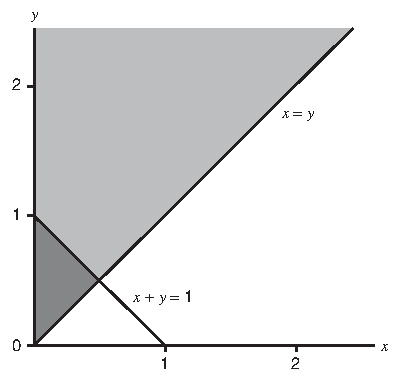
\includegraphics[width=.54\linewidth]{assets/chapter4/fig4-1-1.pdf}
\caption{\autoref{ex:4.1.12} 中的区域}\label{fig:4.1.1}
\end{figure}

\begin{example}[联合概率的计算——II]\label{ex:4.1.12}
再看一个联合 pdf 的例子：令 $f(x,y)=e^{-y}$，$0<x<y<\infty$. 虽然 $e^{-y}$ 不依赖 $x$，但 $f(x,y)$ 显然是 $x$ 的函数，因为使 $f(x,y)$ 非零的集合依赖 $x$. 用示性函数写成
$$f(x,y)=e^{-y}I_{\{(u,v):0<u<v<\infty\}}(x,y),$$
这一点就更清楚了. 为计算 $P(X+Y\ge1)$，可以在集合 $A=\{(x,y):x+y\ge1\}$ 与 $f(x,y)$ 非零区域的交集上对联合 pdf 积分. 画出这些集合，可见该区域是一个无界区域（\autoref{fig:4.1.1} 中较浅的阴影），三条边分别位于直线 $x=y$、$x+y=1$ 和 $x=0$ 上. 为写出合适的积分限，至少需要把它拆成两部分.

在集合 $B=\{(x,y):x+y<1\}$ 与 $f(x,y)$ 非零区域的交集上积分会更容易. 这个交集是由直线 $x=y$、$x+y=1$ 和 $x=0$ 围成的三角形区域（\autoref{fig:4.1.1} 中较深的阴影）. 因此，
$$
\begin{aligned}
P(X+Y\ge1)&=1-P(X+Y<1)=1-\int_0^{1/2}\int_x^{1-x}e^{-y}\,dy\,dx\\
&=1-\int_0^{1/2}(e^{-x}-e^{-(1-x)})\,dx=2e^{-1/2}-e^{-1}.
\end{aligned}
$$
这说明，在这类问题中，为确定恰当的积分限，把相关集合画出来几乎总是有帮助的.
\end{example}
\sourcepageanchor{152}

$(X,Y)$ 的联合概率分布也可以用联合累积分布函数（joint cumulative distribution function，联合 cdf）来完全描述，而不使用联合 pmf 或联合 pdf. 联合 cdf 是定义在所有 $(x,y)\in\mathbb R^2$ 上的函数\index{SI0239@联合}\semanticindexanchor{239:152}
$$F(x,y)=P(X\le x,Y\le y).$$
对离散随机向量而言，联合 cdf 通常不太方便. 但对于连续二元随机向量，像单变量情形一样，有重要关系
$$F(x,y)=\int_{-\infty}^x\int_{-\infty}^y f(s,t)\,dt\,ds.$$
由二元微积分基本定理，在 $f(x,y)$ 的连续点处，
\begin{equation}\label{eq:4.1.3}\index{SI0448@微积分基本定理}
\frac{\partial^2F(x,y)}{\partial x\partial y}=f(x,y).
\end{equation}
当能够求出 $F(x,y)$ 的表达式时，这个关系十分有用：计算混合偏导数即可得到联合 pdf.
